\documentclass[a4paper, 11pt]{article}

\usepackage{graphicx}

\begin{document}

\title {Project X: New Approach to Still Shot Processing}

\author{Graeme Winter}

\maketitle

\section{Problem}

At the moment accurate refinement of still shot data presents problems where
central impacts are used, as the assumption that the full reflection has 
contributed to the centre of mass of the observed spot is manifestly false.
Methods to address this typically rely on estimating some correction factor
based on the crystal mosaicity, but these are inherently dependent on the 
choice of mosaicity model and also are not able to take the \emph{absence}
of a reflection into consideration.

\section{Suggestion}

Given an indexed diffraction pattern, a Miller index may be computed for any 
position on the detector, be this a reflection or no. Of course, most of these
indices will be non-integral, and the index assigned is entirely dependent on 
the current orientation matrix and unit cell. The option however exists to 
compute an ``image'' of the distance to the nearest integral reciprocal lattice
point (relp) or some function of this distance for every
pixel, and compare this with the observed pixel data. If a function is used
which rapidly decreases as the distance from the relp increases, the resulting 
map should look similar to the original diffraction image if the length scale
for the fall off is comparable to the reciprocal space size of the observed
reflections.

This therefore gives the opportunity to compute a penalty function not as the
observed gap between observed and predicted spots, but instead to use the 
similarity of the observed pixel data to the calculated distance function: if
relps are close to reflecting position they should be observed, and if they are
not observed this may be used to guide model improvement.

Proposed penalty function: correlation of calculated distance function with 
observed pixel data - maximising this should result in a good model of the 
data.

For example image 9 (one lattice) this gives an image like:

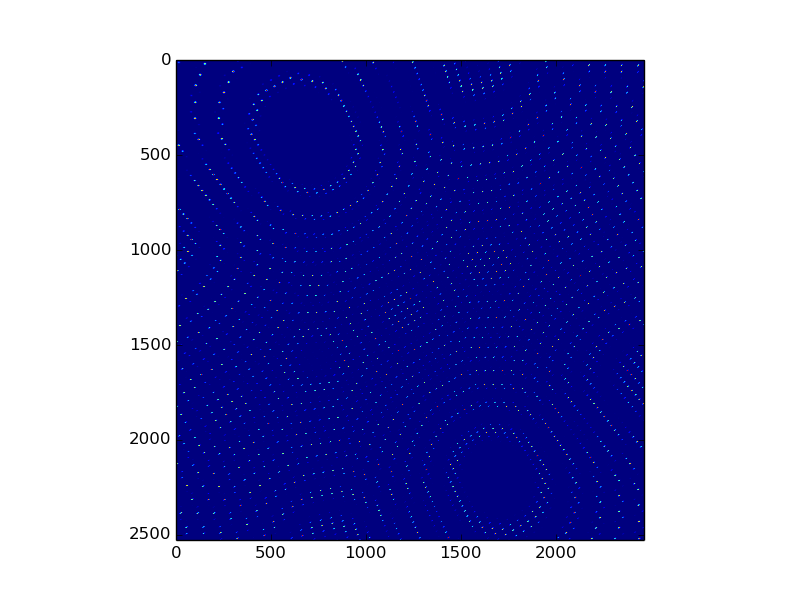
\includegraphics[scale=0.5]{project_x.png}

This was calculated with a 3D Gaussian with $r=0.1$ i.e. corresponding to a 
sphere around each relp - here there are clearly more spots than were measured,
so in this case $r$ is too large. Also spots were only observed to around 
1.8\AA, so some kind of $B$-factor model will be needed.

\section{Issues}

This is computationally expensive to evaluate, particularly with the current 
Python code. Probably impossible to get analytical derivitives. To make function
vary smoothly as the model parameters are changed may require integration of 
the distance function across each pixel rather than taking the central value, 
particularly if the pixels are large when compared with the spot. 

Actually integrating the data following this could use the computed distance 
function as a proxy for the reflection profile, and this would give an 
opportunity to derive a useful scale factor at the same time.

\end{document}

